\section{Core Comunication Facilities}
\subsection{Socket}
Nella programmazione di rete esistono diversi tipi di protocolli tra cui l'\emph{unicast TCP}, l'\emph{unicast UDP} e il \emph{multicast IP}. Per ogni protocollo esiste un RFC che descrive come questi protocolli lavorano in pratica, tuttavia, il problema principale è capire come un programmatore possa trarre vantaggio da questi protocolli. La risposta a questa domanda sono i \textbf{Socket}, comparsi per la prima volta 1982 nel sistema Unix BSD oggi sono disponibili per qualsiasi sistema. I \emph{socket} forniscono un'astrazione comune per la comunicazione interprocesso sia essa di tipo \emph{connection-oriented (TCP)} sia di tipo \emph{connection-less (UDP)}.\\
\subsubsection{I socket in C}
Il flusso di esecuzione di una comunicazione tra due processi segue lo schema in \figurename"\ref{fig:streamsocket} in questo caso si tratta di una comunicazione orientata alla connessione infatti vediamo come il processo \emph{client} (quello a destra) effettui una \texttt{connect()} prima di inviare o ricevere dei dati.
\begin{figure}
\centering
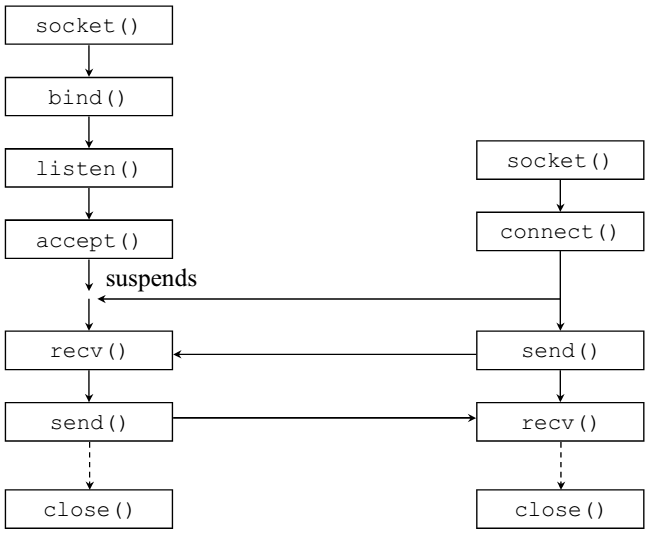
\includegraphics[width=0.7\linewidth]{img/streamsocket}
\caption{Flusso di esecuzione di una comunicazione orientata alla connessione}
\label{fig:streamsocket}
\end{figure}
Vediamo ora due esempi di un client e di un server TCP rispettivamente nel Listato \ref{lst:clienttcp} e nel Listao \ref{lst:servertcp}
\lstinputlisting[language=C,caption={Client TCP},label=lst:clienttcp]{listati/ClientTCP.c}
\lstinputlisting[language=C,caption={Server TCP},label=lst:servertcp]{listati/ServerTCP.c}
Abbiamo visto come funziona una comunicazione orientata alla connessione vediamo ora come funziona invece una comunicazione di tipo \emph{connection-less} mostrata in \figurename"\ref{fig:udpcon}.
\begin{figure}
\centering
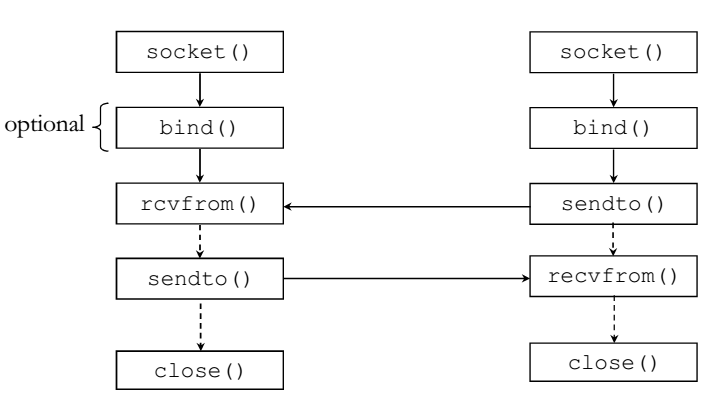
\includegraphics[width=0.7\linewidth]{img/udpcon}
\caption{Flusso di esecuzione di una comunicazione senza connessione}
\label{fig:udpcon}
\end{figure}
Come vediamo in questo caso non è necessario effettuare l'\texttt{accept} ne la \texttt{connect} in quanto i messaggi sono inviati direttamente, questo meccanismo è più rapido del precedente ma risulta essere meno sicuro.
\subsubsection{I socket in Java}
In Java l'approccio ai \emph{socket} è simile al C risulta tuttavia molto più semplice. Esistono cique classi principali fornite dal \emph{package} \texttt{java.net} queste classi sono:
\begin{itemize}
\item \texttt{InetAddress:} fornisce i metodi per ottentere l'indirizzo di un host dato il suo \emph{hostname} e vice versa
\item \texttt{ServerSocket:} utilizzata dal server per accettare le connessioni in ingresso.
\item \texttt{Socket:} la classe principale utilizzata per la comunicazione
\item \texttt{DatagramPacket:} classe utilizzata per inviare messaggi attraverso un  \texttt{DatagramSocket}
\item \texttt{DatagramSocket:} classe utilizzata per l'invio e la ricezione di messaggi senza l'ausilio di una connessione
\end{itemize}
Un esempio di un client e di un server TCP in Java è mostrato rispettivamente nel Listato \ref{lst:javaclient} e nel Listato \ref{lst:javaserver}.
Vediamo come in java la comunicazione avvenga tramite input e output stream associati ad una socket.
\lstinputlisting[language=Java,caption={Client TCP in Java},label=lst:javaclient]{listati/TCPClient.java}
\lstinputlisting[language=Java,caption={Server TCP in Java},label=lst:javaserver]{listati/TCPServer.java}
Le classi \texttt{ObjectInputStream} e \texttt{ObjectOutputStream} permettono di leggere e scrivere su di uno stream serializzato; per essere trasmesso su questo tipo di stream un oggetto deve essere serializzabile ovvero deve implementare l'interfaccia \texttt{Serializable}. La serializzazione permette una \emph{copia profonda} di un oggetto. Un programmatore può impedire la serializzazione di un oggetto dichiarandolo di tipo \texttt{transient}.
\subsubsection{IP Multicast}
Il \textbf{multicast IP} è un protocollo di rete che permette la consegna di pacchetti UDP a molti destinatari contemporaneamente. Per implementare tale protocollo solitamente si riservano degli indirizzi IP di classe D per i gruppi \emph{multicast}.\\
I componenti interessati a ricevere dei messaggi inviati in un gruppo devono effettuare una \emph{join} a tale gruppo, non è necessario, invece, unirsi al gruppo per inviare un messaggio indirizzato ad un determinato gruppo.\\
Java fornisce una sottoclasse della classe \texttt{DatagramSocket} denominata \texttt{MulticastSocket} per implementare in modo semplice il multicast; questa classe aggiunge due metodi alla classe \texttt{DatagramSocket} che sono il \texttt{joinGroup} e il \texttt{leaveGroup}.
\subsection{Remote procedure call}
Con lo sviluppo della programmazione il problema che si è presentato è che l'interazione tra client e server avveniva sempre tramite le primitive di I/O del sistema, questo rendeva le applicazioni difficili da sviluppare. L'idea di \emph{Sun Microsystems} è stata quella di permettere l'accesso remoto attraverso un meccanismo ben conosciuto ovvero quello delle chiamate a procedura come mostrato in \figurename \ref{fig:rpc}.
\begin{figure}[tb]
\centering
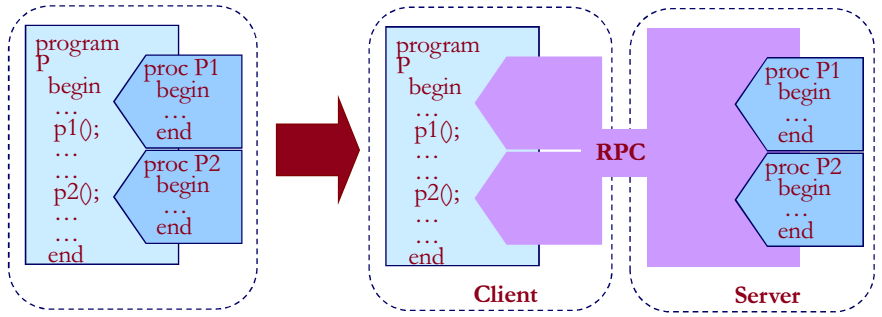
\includegraphics[width=0.7\linewidth]{img/rpc}
\caption{Modello di chiamata a procedura remota}
\label{fig:rpc}
\end{figure}
Tuttavia questo modello comporta alcuni problemi soprattutto per quanto riguarda il passaggio dei parametri. Il primo problema dovuto al passaggio dei parametri è quello della conversione di strutture dati complesse come oggetti o \texttt{struct} in uno stream di byte sequenziale, tale problema è chiamato \emph{serializzazione}. Il secondo problema che si presenta è il fatto che un sistema host potrebbe usare una rappresentazione dei dati differente ed è quindi necessaria una conversione, tale problema è chiamato \emph{marshalling}.\\
I middleware forniscono supporto automatico per risolvere questi problemi, il marshaling e la serializzazione sono implementati automaticamente e entrano a far parte dello stub; inoltre permettono un'indipendenza dal linguaggio in quanto le procedure vengono rappresentate tramite un \emph{Interface Definition Language} (IDL).\\
L'\emph{interface definition language} alza il livello di astrazione della definizione del servizio separando l'\emph{interfaccia} del servizio dalla sua \emph{implementazione}. I vantaggi di questa tecnica è quello di definire un servizio indipendentemente dal linguaggio utilizzato per implementarlo, inoltre, l'utilizzo di un IDL definito formalmente permette la generazione automatica delle interfacce nel linguaggio target.\\
Sun Microsystem RPC anche chiamata ONC RPC è lo standard \emph{de facto} psu internet, il formato dei dati è specificato da un XDR (\emph{eXternal Data Representation}) che, nato come un linguaggio di rappresentazione dei dati, attualmente si è evoluto in un vero e proprio IDL. Il livello di trasporto può utilizzare sia il TCP che l'UDP, il passaggio di parametri è consentito solo tramite copia ed un solo valore di input e uno di output sono permessi.\\
Esiste un altro standard per le RPC, questo standard è il \emph{Distributed Computing Environment} il quale è un insieme di specifiche e riferimenti ad implementazioni, questo standard fornisce specifiche per i servizi di alto livello come \emph{directory service} o \emph{distributed time service}; la sicurezza inoltre è fornita attraverso \emph{Kerberos}. Il sistema di RPC di Microsoft DCOM e .Net sono basati su DCE.\\
Il funzionamento delle Sun RPC è mostrato in \figurename"\ref{fig:sunrpc} nel quale partendo da il file di specifica \texttt{rdate.x} mostrato nel Listato \ref{lst:rdate} e mediante l'invocazione del programma \texttt{rpcgen} si vengono a creare i file necessari per la stesura dei programmi client e server.
\begin{figure}
\centering
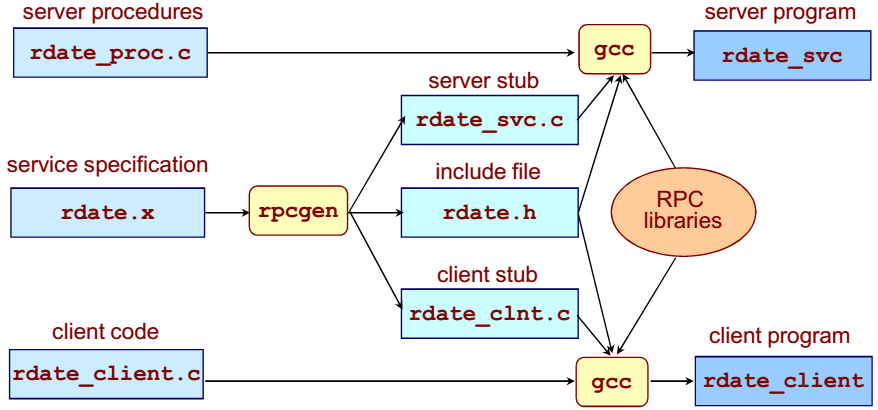
\includegraphics[width=0.7\linewidth]{img/sunrpc}
\caption{Funzionamento delle Sun RPC}
\label{fig:sunrpc}
\end{figure}
\begin{lstlisting}[language=IDL,caption="Esempio di file rdate.x",label=lst:rdate]
program RDATE_PROG {
    version RDATE_VERS {
        long BIN_DATE(void) = 1;	/* procedure number */
        string STR_DATE(long) = 2;	/* procedure number */
    } = 1;							/* version number   */
}= 0x20000001;						/* program number   */
\end{lstlisting}
Come detto il passaggio di parametri è consentito solo tramite copia, per molti linguaggi questo non è un problema in quanto non è supportato nemmeno a livello di linguaggio in altri contesti tuttavia è possibile utilizzare delle chiamate per \emph{valore/risultato} al posto della chiamata per riferimento.
\subsection{Remote method invocation}
La \emph{Remote Method Invocation} (RMI) sfrutta la stessa idea della RPC ma si basa su costruzioni di programmazione differenti, lo scopo è quello di ottenere i vantaggi di una programmazione Object-Oriented solamente in un contesto distribuito. Un'importante differenza rispetto alle RPC è che nelle RMI è possibile il passaggio di oggetti per riferimento, questo richiede il mantenimento delle relazioni con gli alias. In molti casi le RMI sono sviluppate su un livello di RPC.\\
Nelle RPC l'IDL separa l'interfaccia dall'implementazione, questa separazione è alla base dei principi di programmazione OO, è naturale posizionare l'interfaccia di un oggetto su di un host e l'implementazione su di un altro.\\
\subsubsection{Java RMI}
JAva RMI è il più semplice tra i moderni sistemi ad oggetti distribuiti più diffusi, esso si concentra solamente sulle chiamate di metodi remote il resto dei servizi è fornito da altri componenti della famiglia Java, permette di effettuare il download delle classi, di avere dei proxies dinamici.\\
Il concetto di interfaccia Java assume un nuovo ruolo con la distribuzione, un \emph{oggetto remoto} deve implementare un'interfaccia che estende \texttt{java.rmi.Remote} come nell'esempio del Listato \ref{lst:extendsRemote}
\begin{lstlisting}[language=Java,caption="Esempio di interfaccia remota",label=lst:extendsRemote]
import java.rmi.*
public interface AccountServer extends Remote {
	Account getAccount (int num) throws RemoteException;
}
\end{lstlisting}
Implementare un interfaccia remota non è sufficiente per accettare delle chiamate remote, per fare ciò è necessario \emph{esportare} l'oggetto.
Questo può essere fatto automaticamente nel costruttore se la classe deriva da \texttt{java.rmi.server.RemoteObject} come nel caso di \texttt{UnicastRemoteObject} oppure staticamente invocando il metodo \texttt{UnicastRemoteObject.exportObject}.\\
Per ottenere un riferimento ad un oggetto remoto esistono due modi, attraverno il passaggio di parametri o come valore di ritorno oppure interrogando esplicitamente un servizio di \emph{lookup} denominato \texttt{rmiregistry}. In entrambi i casi il riferimento all'oggetto remoto contiene lo stub del client ovvero implementa l'interfaccia remota, istanzia il \texttt{RemoteStub}. Una volta acquisito il riferimento remoto esso è indistinguibile da uno locale.\\
RMI non maschera completamente la distribuzione, notiamo la presenza di eccezioni ed interfacce remote, questo è il risultato di una precisa scelta progettuale per distingure un interazione locale da una remota. RMI inoltre è uno strumento poco potente rispetto agli altri sistemi ad oggetti distribuiti, tuttavia altri componenti Java sono costruiti su di esso come JavaEE.